\chapter{Design}
\label{ch:design}
\section{Introduction}

\section{Methodology}

\section{Technologies}
This section outlines the technologies that will be used for the project, and gives a justification for why each technology will be used. This includes programming languages, web frameworks, and libraries.

\subsection{Programming Languages}
\label{sec:lang}
Based on the research in Chapter~\ref{ch:lit}, there are a number of candidates for developing a chatbot system. The following table summarises the main features of each, and how they might be effective for this project.

\begin{table}[h]
	\centering
	\begin{tabularx}{\textwidth}{{@{}lXXX@{}}}
		\toprule
		& Java & Python & Ruby \\
		\midrule
		Description 
			& Popular object-oriented language used in many enterprise solutions.
			& A well-established language in data science and machine learning communities.
			& Interpreted language commonly combined with Rails in web applications. \\
		Advantages
			& Popular language with a large community.
			
			Java Virtual Machine (JVM) allows for integrated cross-platform support.
			
			& Abundant range of libraries for machine learning.
			
			& 
				
	\end{tabularx}
	\caption{Comparison of programming language candidates.}
	\label{tab:lang}
\end{table}

It is clear that this system could be implemented in any language \hilight{...}

Therefore, the project will be implemented in Java, mainly because of my familiarity with the language.\hilight{continue}


\subsection{Web Frameworks}
In the case of Java, there are several web frameworks that can be used to handle webpage design, routing, and configuration.

\subsection{Chatbot Model}


\subsection{Libraries}

\newpage
\section{Architecture}
\subsection{System Design}
The following diagram shows the overall system design for the proposed solution.
\hilight{diagram}

\begin{figure}[h]
	\begin{center}
		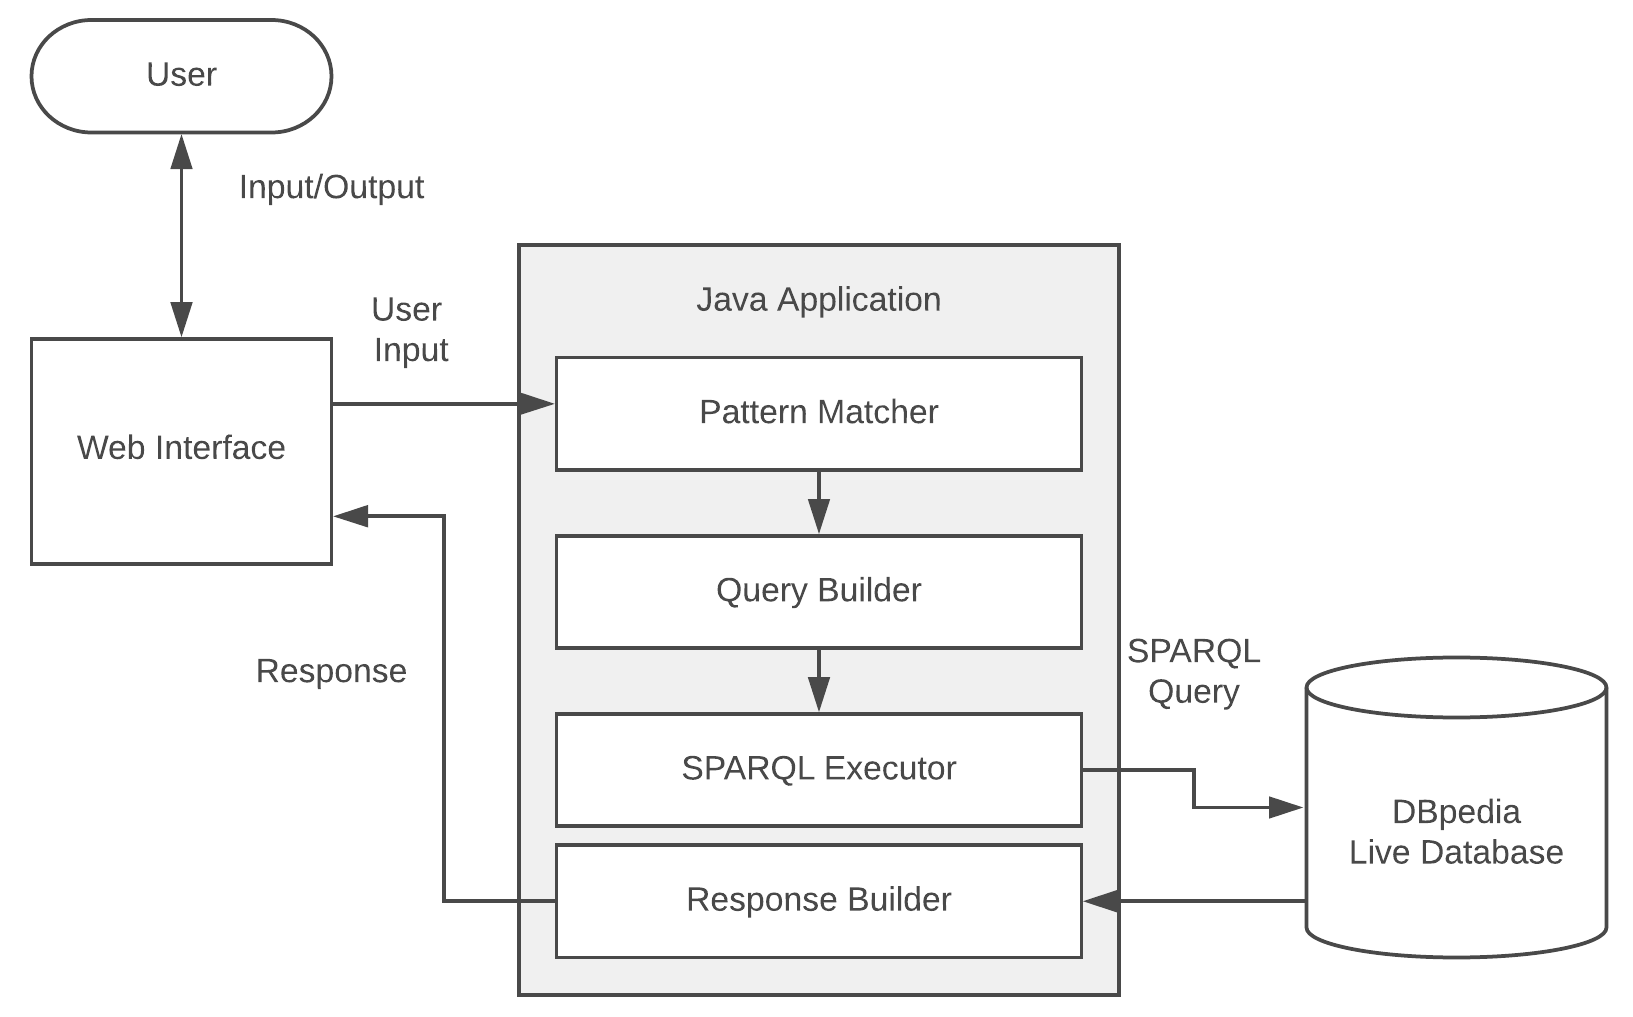
\includegraphics[width=\textwidth]{design_system}
	\end{center}
	\caption{Overview of architecture of the system.}
	\label{fig:design_system}
\end{figure}

\newpage
\subsection{Activity}
Figure~\ref{fig:design_activity} shows the flow of events through the system, from the user input to the resulting output. \hilight{continue}

\begin{figure}[h]
	\begin{center}
		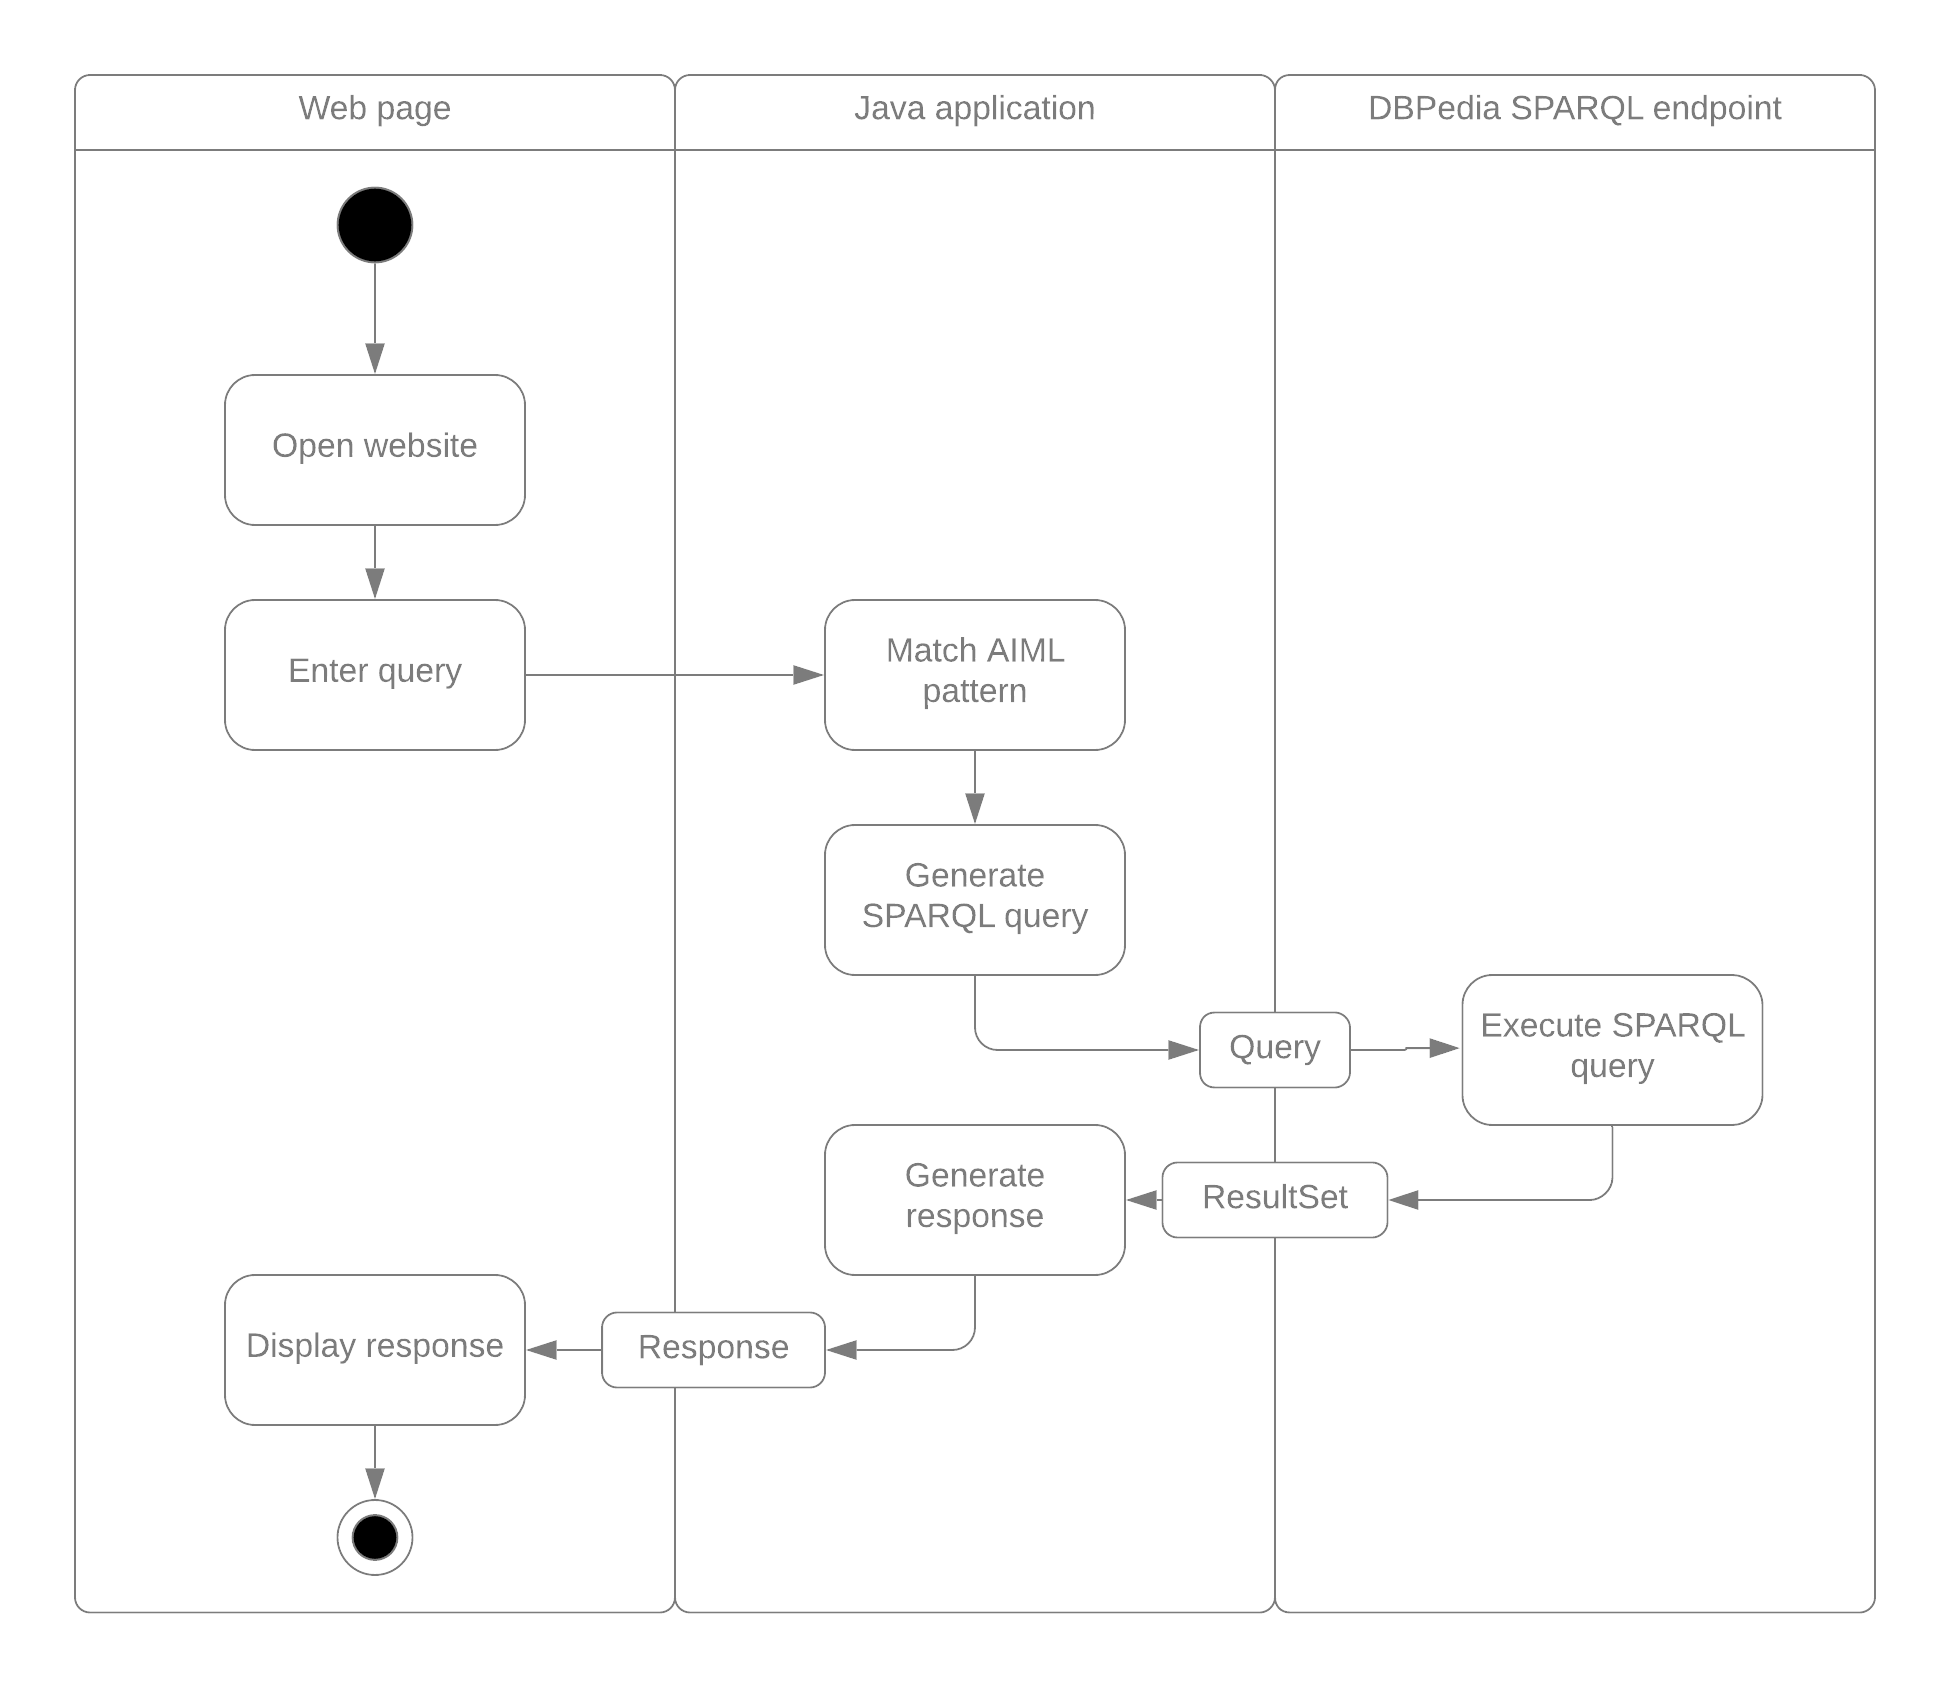
\includegraphics[width=\textwidth]{design_activity}
	\end{center}
	\caption{UML Activity diagram.}
	\label{fig:design_activity}
\end{figure}

\newpage
\section{User Interface}
The proposed system will be a web application for a number of reasons. Firstly, it will allow testers to easily access the application without having to download any files. It also allows for easy customisation using HTML and CSS. The alternative would be a text-based user interface (TUI), which would require less configuration, but will be limited in terms of rendering images, links, and other elements. It will be beneficial to use a TUI during development, as this would allow the system to be built and debugged quickly. Figure~\ref{fig:design_ui} shows the expected web interface design for the system.

\begin{figure}[h]
	\begin{center}
		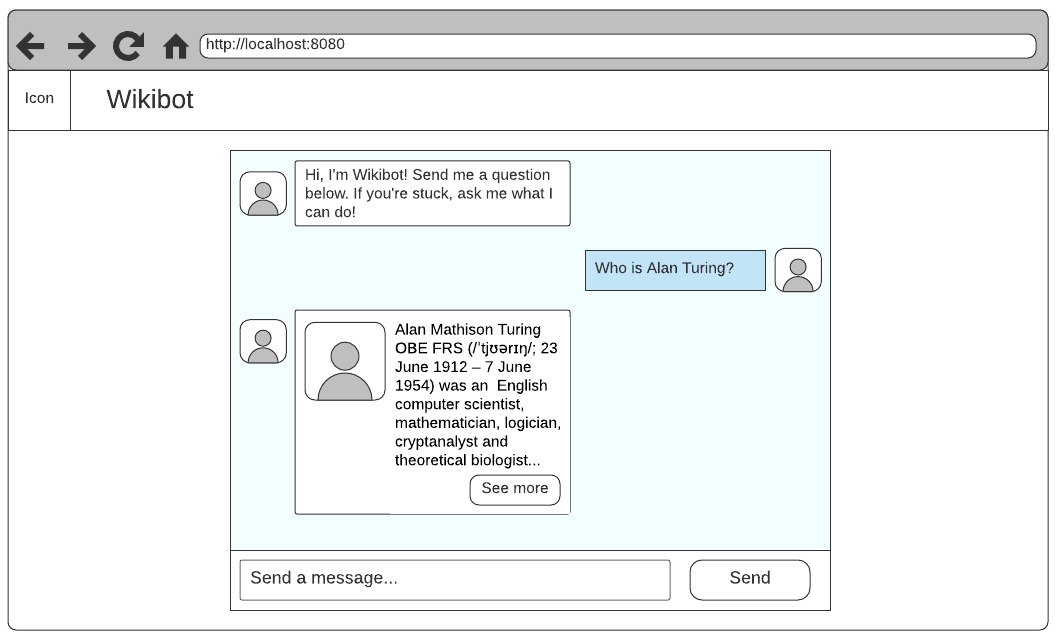
\includegraphics[width=\textwidth]{design_ui}
	\end{center}
	\caption{Web UI interface design.}
	\label{fig:design_ui}
\end{figure}

\section{Data}